\documentclass[13pt]{article}
\usepackage[T1]{fontenc}
\usepackage{graphicx}
\title{Diagram stanów}
\author{Piotr Popis}
\date{Maj 2020}
\begin{document}
\begin{titlepage}
\maketitle
\end{titlepage}
\section{Stany główne}
\subsection{Diagram}
\hspace*{-3.5cm}                                                           
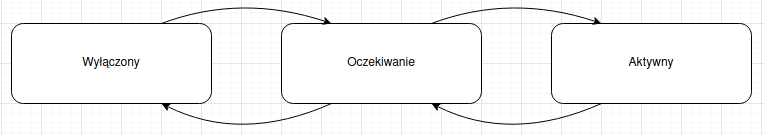
\includegraphics[scale=.7]{state_full.png}
\subsection{Opis}
Color Sorting Machine może znajdować się w trzech głównych stanach: wyłączony, oczekujący i aktywny. \\
 \hspace*{1cm} Aby przejść ze stanu wyłączony do stanu oczekującego musimy (po podłączeniu zasilacza oczywiście) włączyć przycisk ON. Wtedy wszystkie serwa resetują się do pozycji zerowej, gdyby działanie programu zostało przerwane podczas działania maszyny i serwa utknęły w pozycji x na przykład w wyniku odcięcia zasilania. System oczekuje na obiekt analizy. Aby wrócić do stanu wyłączony musimy wcisnąć przycisk OFF.\\
\hspace*{1cm}
By ze stanu oczekiwania przejść w stan aktywności musimy wsadzić przedmiot do podajnika i uruchomić działanie przyciskiem start na panelu. Powrót do stanu oczekiwania następuje po wykonaniu pełnej sekwencji( algorytmu przetwarzania wejść na wyjścia).\\
\section{Analiza}
\section{Opis}
Zasadniczo stan czuwania oraz stan wyłączony są dość oczywiste i opis ogólny jest mniej więcej równomierny z szczegółowym( nie ma co tam za bardzo opisywać). W stanie wyłączenia system nie działa nie pracuje, nie ma dopływu prądu. W stanie czuwania system przepływa prąd, ale system nie wykonuje żadnych zadań( tasks) prócz oczekiwania na wprowadzenie. Po wprowadzeniu przechodzimy do stanu Aktywności - stan aktywności jest zdecydowanie bardziej złożony - składa się z innych podstanów, które chciałbym przeanalizować.
\subsection{Diagram stanów w stanie aktywności}
\hspace*{-2.0cm}                                                           
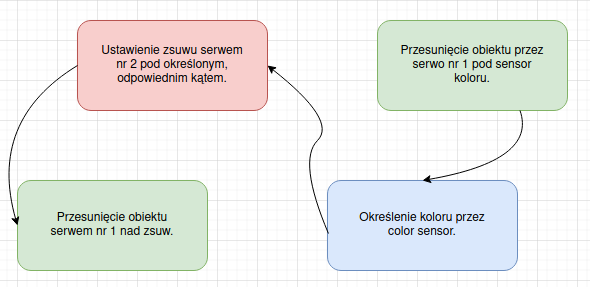
\includegraphics[scale=0.8]{activity.png}
\section{Diagram Szczegółowy}
W zasadzie z każdego stanu powinno być przejście do wyłączonego, ponieważ w każdym momencie możemy wcisnąć przycisk Off.\\
\hspace*{-2.0cm}    
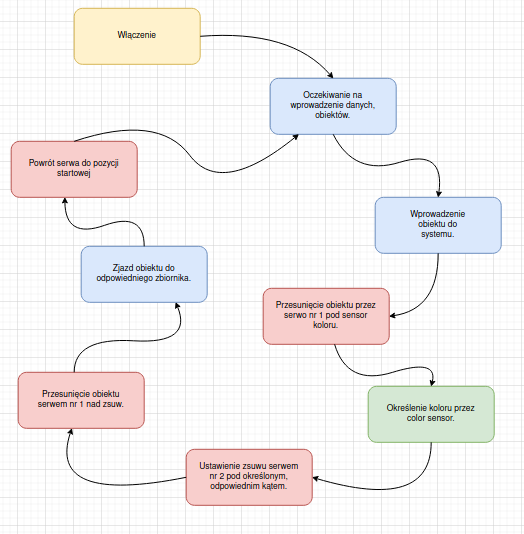
\includegraphics[scale=0.8]{full.png}
\end{document}